% Options for packages loaded elsewhere
\PassOptionsToPackage{unicode}{hyperref}
\PassOptionsToPackage{hyphens}{url}
%
\documentclass[
]{article}
\usepackage{amsmath,amssymb}
\usepackage{iftex}
\ifPDFTeX
  \usepackage[T1]{fontenc}
  \usepackage[utf8]{inputenc}
  \usepackage{textcomp} % provide euro and other symbols
\else % if luatex or xetex
  \usepackage{unicode-math} % this also loads fontspec
  \defaultfontfeatures{Scale=MatchLowercase}
  \defaultfontfeatures[\rmfamily]{Ligatures=TeX,Scale=1}
\fi
\usepackage{lmodern}
\ifPDFTeX\else
  % xetex/luatex font selection
\fi
% Use upquote if available, for straight quotes in verbatim environments
\IfFileExists{upquote.sty}{\usepackage{upquote}}{}
\IfFileExists{microtype.sty}{% use microtype if available
  \usepackage[]{microtype}
  \UseMicrotypeSet[protrusion]{basicmath} % disable protrusion for tt fonts
}{}
\makeatletter
\@ifundefined{KOMAClassName}{% if non-KOMA class
  \IfFileExists{parskip.sty}{%
    \usepackage{parskip}
  }{% else
    \setlength{\parindent}{0pt}
    \setlength{\parskip}{6pt plus 2pt minus 1pt}}
}{% if KOMA class
  \KOMAoptions{parskip=half}}
\makeatother
\usepackage{xcolor}
\usepackage[margin=1in]{geometry}
\usepackage{color}
\usepackage{fancyvrb}
\newcommand{\VerbBar}{|}
\newcommand{\VERB}{\Verb[commandchars=\\\{\}]}
\DefineVerbatimEnvironment{Highlighting}{Verbatim}{commandchars=\\\{\}}
% Add ',fontsize=\small' for more characters per line
\usepackage{framed}
\definecolor{shadecolor}{RGB}{248,248,248}
\newenvironment{Shaded}{\begin{snugshade}}{\end{snugshade}}
\newcommand{\AlertTok}[1]{\textcolor[rgb]{0.94,0.16,0.16}{#1}}
\newcommand{\AnnotationTok}[1]{\textcolor[rgb]{0.56,0.35,0.01}{\textbf{\textit{#1}}}}
\newcommand{\AttributeTok}[1]{\textcolor[rgb]{0.13,0.29,0.53}{#1}}
\newcommand{\BaseNTok}[1]{\textcolor[rgb]{0.00,0.00,0.81}{#1}}
\newcommand{\BuiltInTok}[1]{#1}
\newcommand{\CharTok}[1]{\textcolor[rgb]{0.31,0.60,0.02}{#1}}
\newcommand{\CommentTok}[1]{\textcolor[rgb]{0.56,0.35,0.01}{\textit{#1}}}
\newcommand{\CommentVarTok}[1]{\textcolor[rgb]{0.56,0.35,0.01}{\textbf{\textit{#1}}}}
\newcommand{\ConstantTok}[1]{\textcolor[rgb]{0.56,0.35,0.01}{#1}}
\newcommand{\ControlFlowTok}[1]{\textcolor[rgb]{0.13,0.29,0.53}{\textbf{#1}}}
\newcommand{\DataTypeTok}[1]{\textcolor[rgb]{0.13,0.29,0.53}{#1}}
\newcommand{\DecValTok}[1]{\textcolor[rgb]{0.00,0.00,0.81}{#1}}
\newcommand{\DocumentationTok}[1]{\textcolor[rgb]{0.56,0.35,0.01}{\textbf{\textit{#1}}}}
\newcommand{\ErrorTok}[1]{\textcolor[rgb]{0.64,0.00,0.00}{\textbf{#1}}}
\newcommand{\ExtensionTok}[1]{#1}
\newcommand{\FloatTok}[1]{\textcolor[rgb]{0.00,0.00,0.81}{#1}}
\newcommand{\FunctionTok}[1]{\textcolor[rgb]{0.13,0.29,0.53}{\textbf{#1}}}
\newcommand{\ImportTok}[1]{#1}
\newcommand{\InformationTok}[1]{\textcolor[rgb]{0.56,0.35,0.01}{\textbf{\textit{#1}}}}
\newcommand{\KeywordTok}[1]{\textcolor[rgb]{0.13,0.29,0.53}{\textbf{#1}}}
\newcommand{\NormalTok}[1]{#1}
\newcommand{\OperatorTok}[1]{\textcolor[rgb]{0.81,0.36,0.00}{\textbf{#1}}}
\newcommand{\OtherTok}[1]{\textcolor[rgb]{0.56,0.35,0.01}{#1}}
\newcommand{\PreprocessorTok}[1]{\textcolor[rgb]{0.56,0.35,0.01}{\textit{#1}}}
\newcommand{\RegionMarkerTok}[1]{#1}
\newcommand{\SpecialCharTok}[1]{\textcolor[rgb]{0.81,0.36,0.00}{\textbf{#1}}}
\newcommand{\SpecialStringTok}[1]{\textcolor[rgb]{0.31,0.60,0.02}{#1}}
\newcommand{\StringTok}[1]{\textcolor[rgb]{0.31,0.60,0.02}{#1}}
\newcommand{\VariableTok}[1]{\textcolor[rgb]{0.00,0.00,0.00}{#1}}
\newcommand{\VerbatimStringTok}[1]{\textcolor[rgb]{0.31,0.60,0.02}{#1}}
\newcommand{\WarningTok}[1]{\textcolor[rgb]{0.56,0.35,0.01}{\textbf{\textit{#1}}}}
\usepackage{longtable,booktabs,array}
\usepackage{calc} % for calculating minipage widths
% Correct order of tables after \paragraph or \subparagraph
\usepackage{etoolbox}
\makeatletter
\patchcmd\longtable{\par}{\if@noskipsec\mbox{}\fi\par}{}{}
\makeatother
% Allow footnotes in longtable head/foot
\IfFileExists{footnotehyper.sty}{\usepackage{footnotehyper}}{\usepackage{footnote}}
\makesavenoteenv{longtable}
\usepackage{graphicx}
\makeatletter
\def\maxwidth{\ifdim\Gin@nat@width>\linewidth\linewidth\else\Gin@nat@width\fi}
\def\maxheight{\ifdim\Gin@nat@height>\textheight\textheight\else\Gin@nat@height\fi}
\makeatother
% Scale images if necessary, so that they will not overflow the page
% margins by default, and it is still possible to overwrite the defaults
% using explicit options in \includegraphics[width, height, ...]{}
\setkeys{Gin}{width=\maxwidth,height=\maxheight,keepaspectratio}
% Set default figure placement to htbp
\makeatletter
\def\fps@figure{htbp}
\makeatother
\setlength{\emergencystretch}{3em} % prevent overfull lines
\providecommand{\tightlist}{%
  \setlength{\itemsep}{0pt}\setlength{\parskip}{0pt}}
\setcounter{secnumdepth}{-\maxdimen} % remove section numbering
\ifLuaTeX
  \usepackage{selnolig}  % disable illegal ligatures
\fi
\usepackage{bookmark}
\IfFileExists{xurl.sty}{\usepackage{xurl}}{} % add URL line breaks if available
\urlstyle{same}
\hypersetup{
  pdftitle={Predicting Bike Share Ridership based on Weather Data in Seattle},
  pdfauthor={Joey Rodriguez and Daniel Bhatti},
  hidelinks,
  pdfcreator={LaTeX via pandoc}}

\title{Predicting Bike Share Ridership based on Weather Data in Seattle}
\author{Joey Rodriguez and Daniel Bhatti}
\date{2024-11-22}

\begin{document}
\maketitle

\section{Introduction}\label{introduction}

Cycle share has launched in many U.S. cities since its introduction in
Washington, D.C. in 2010 (1). One iteration of cycle share was Pronto!
in downtown Seattle, Washington. From 2014 to 2017, 500 Pronto! bikes
operated across 54 stations on the ithsmus. The City of Seattle, in
partnership with Socratica, collected system data during the operating
window and made it public via its open data platform. Pronto! fell short
of the success realized by other bike schemes in the U.S. like Capital
Bikeshare, Philly's Indego, and NYC's CitiBike. Researchers have used
system data to conduct a post-mortem analysis on Pronto! as dockless
bike share schemes like Lime Scooters filled the void left by Pronto
(2). In this paper, we will investigate the relationship between weather
in the service area and daily ridership. In particular, we want to
predict daily ridership based on the weather data.

The data were downloaded from Kaggle (3). The file \texttt{trip.csv}
contains data on each trip from 13 October 2014 to 31 March 2017, or 901
days. Each case in this dataset is a trip, and there were 275,091 trips
over the 901 days. The relevant variables from the original 12 in this
dataset are the response variables \texttt{start\_time} (day and time
trip started, in PST) and \texttt{trip\_duration} (time of trip in
seconds). In the file \texttt{weather.csv.xls}, a single case
corresponds to a single day. This file contains the weather data for
each day from 13 October 2014 to 31 August 2016, or 689 days. That is,
the dates covered by the \texttt{weather} data set are a proper subset
of the dates covered by the \texttt{trip} data set. Each day has 21
variables describing its weather. After merging these data sets and
creating some of our own variables, we move on to exploratory data
analysis for the response variables and predictors. This exploration
informed our choice for our final model.

{[}INSERT PARAGRAPH SUMMARIZING CONCLUSIONS FROM THE RESEARCH{]}

\section{Exploratory Data Analysis}\label{exploratory-data-analysis}

\subsection{Data Cleaning}\label{data-cleaning}

The \texttt{trip} data frame contains 275,091 cases (or rides) and 12
variables describing each ride. The weather data frame contains 689
cases (or days) and 21 variables describing the weather that day.
Ultimately, our goal is to join these two data frames. We began by
aggregating trip data for each day we have data for. From the
\texttt{trip} data frame, we created a new data frame called
\texttt{ridership} that aggregates trips by day. At the end of this,
\texttt{ridership} has 901 rows (days) and 3 columns (variables):
\texttt{count}, \texttt{tripduration}, and \texttt{day\_number}. Because
the \texttt{trip} data covers 212 days after the last observation in the
\texttt{weather} data, we want to keep only the observations in
\texttt{trip} that match the observations in the smaller data frame,
\texttt{weather}. We created our final data frame, \texttt{df}, by left
joining weather and ridership by \texttt{day\_number}. The final data
frame contains 689 rows (days) and 25 columns (variables). The variable
names are listed in a table below with brief descriptions.

\begin{longtable}[]{@{}
  >{\raggedright\arraybackslash}p{(\columnwidth - 2\tabcolsep) * \real{0.3214}}
  >{\raggedright\arraybackslash}p{(\columnwidth - 2\tabcolsep) * \real{0.6786}}@{}}
\caption{Variable Descriptions (689 rows, 25 columns)}\tabularnewline
\toprule\noalign{}
\begin{minipage}[b]{\linewidth}\raggedright
Variable
\end{minipage} & \begin{minipage}[b]{\linewidth}\raggedright
Description
\end{minipage} \\
\midrule\noalign{}
\endfirsthead
\toprule\noalign{}
\begin{minipage}[b]{\linewidth}\raggedright
Variable
\end{minipage} & \begin{minipage}[b]{\linewidth}\raggedright
Description
\end{minipage} \\
\midrule\noalign{}
\endhead
\bottomrule\noalign{}
\endlastfoot
Max\_Temperature\_F & Maximum temperature (°F) recorded that day \\
Mean\_Temperature\_F & Mean temperature (°F) recorded that day \\
Min\_TemperatureF & Minimum temperature (°F) recorded that day \\
Max\_Dew\_Point\_F & Maximum dew point (°F) recorded that day \\
MeanDew\_Point\_F & Mean dew point (°F) recorded that day \\
Min\_Dewpoint\_F & Minimum dew point (°F) recorded that day \\
Max\_Humidity & Maximum humidity (\%) recorded that day \\
Mean\_Humidity & Mean humidity (\%) recorded that day \\
Min\_Humidity & Minimum humidity (\%) recorded that day \\
Max\_Sea\_Level\_Pressure\_In & Maximum sea-level pressure in inches
recorded that day \\
Mean\_Sea\_Level\_Pressure\_In & Mean sea-level pressure in inches
recorded that day \\
Min\_Sea\_Level\_Pressure\_In & Minimum sea-level pressure in inches
recorded that day \\
Max\_Visibility\_Miles & Maximum visibility in miles recorded that
day \\
Mean\_Visibility\_Miles & Mean visibility in miles recorded that day \\
Min\_Visibility\_Miles & Minimum visibility in miles recorded that
day \\
Max\_Wind\_Speed\_MPH & Maximum wind speed in miles per hour recorded
that day \\
Mean\_Wind\_Speed\_MPH & Mean wind speed in miles per hour recorded that
day \\
Max\_Gust\_Speed\_MPH & Maximum gust speed in miles per hour recorded
that day \\
Precipitation\_In & Precipitation in inches recorded that day \\
Events & Weather events (e.g., Rain, Snow) that occurred that day \\
temp\_range & Temperature range (Max\_Temperature\_F -
Min\_TemperatureF) \\
date & Date of the observation \\
day\_number & Days since 12 October 2014 \\
total\_trips & Total trips recorded that day \\
total\_durations & Total duration of all trips recorded that day in
seconds \\
average\_durations & Average ride duration for that day \\
\end{longtable}

Notice that some variables in our data dictionary were created from
others:

\begin{itemize}
\item \texttt{temp\_range} was created by the difference: \texttt{Max\_Temperature\_F} - \texttt{Min\_TemperatureF}
\item \texttt{date} is in the format \texttt{"\%m/\%d/\%Y"}, because each trip was originally in the format \texttt{"\%m/\%d/\%Y \%H:\%M"}
\item \texttt{day\_number} are the days since 12 October 2014, the first day of observation
\item \texttt{total\_trips} are the total trips recorded for that day
\item \texttt{total\_durations} are the total durations for all trips that day
\item \texttt{avg\_durations} are the average durations for a trip each day
\end{itemize}

\subsection{Selecting the Response
Variable}\label{selecting-the-response-variable}

The three candidates for a good response variable were created from the
\texttt{trip.csv} data set, described in the \texttt{ridership} data
frame, and merged into our final data frame: \texttt{total\_trips},
\texttt{trip\_durations}, and \texttt{avg\_durations}. We briefly
discuss the merits of each response variable before a quantitative
judgement:

\begin{itemize}
\item \texttt{total\_trips} is the most intuitive measure for bike ridership on a given day. It directly answers the question ``How many trips were there?'' for a given day. It gives us a picture of how willing people in the service area were to hop on a bike.
\item \texttt{total\_durations} gives a more complete picture for the ridership on a given day. Once a rider hopped on a bike, how long did they ride before docking it? This gives us a picture of how willing riders in the service area were to stay on their bikes.
\item \texttt{avg\_durations} controls for the interaction between bike ridership and ridership durations. By dividing total ridership over total durations, we understand the willingness of those in the service area to both picking up a bike and keep riding on that bike.
\end{itemize}

The figure below plots daily bike ridership in Seattle, with the total
rides taken each day in blue circles and the sum of the durations of the
rides taken each day in red triangles. This figure suggests that
outliers in total riders tend to coincide with outliers in ride
durations. For instance, the day with the highest bike riders -- 941 on
Sunday, April 20, 2015 -- was also the day with the second highest sum
of ride durations (359.7 hours). It's not clear from lookup what caused
bike ridership to be so high on this day; like much of the data we
gather from the real world, this result was influenced by many factors
that day.

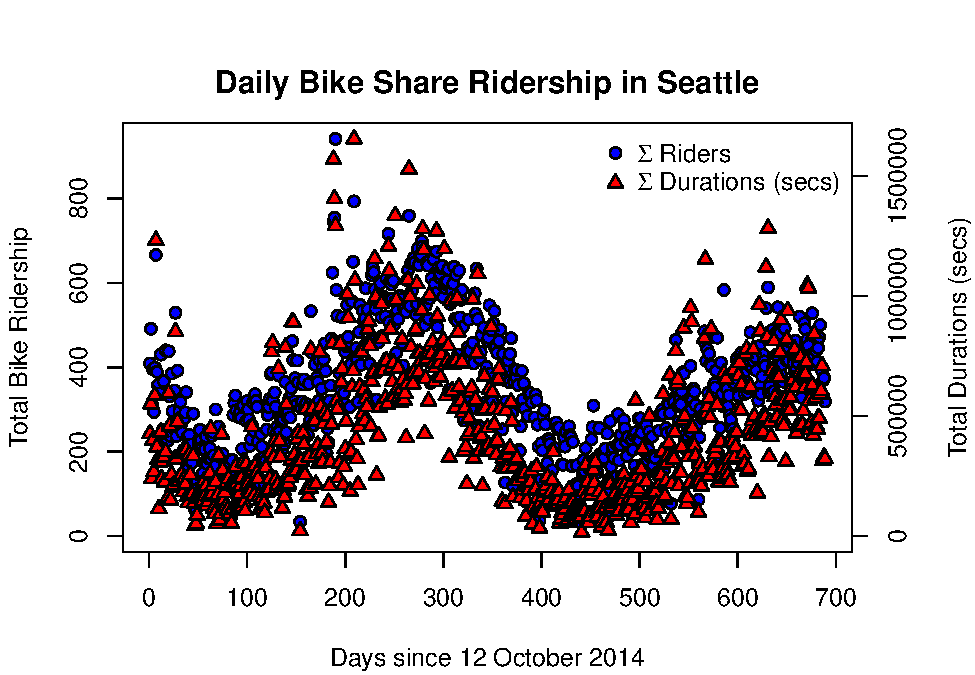
\includegraphics{MATH361_Rough_Draft_files/figure-latex/plot_y-1.pdf}

36 days earlier on Sunday, March 15, 2015 was the second-wettest March
day on record in the Puget Sound Region (SOURCE). The rain was so severe
that a mudslide occured in Western Seattle. Knowing this, you'd expect
March 15 to have been a bad day for cycling. Only 34 trips took place on
this day with a combined ride duration of just 6.3 hours. This was the
second worst day for cycling behind Sunday, December 27, 2015 with just
30 trips and 4.5 hours. The coincidence between trips and durations
explains the flattening of the data -- the decline in variation from the
mean -- once we compute the average ride durations per day. We choose to
skip a visualization of the average each day to visualizing the
normality of the data.

We note (i) that \texttt{total\_trips} and \texttt{total\_durations} are
highly correlated (\textgreater0.82), (ii) that average durations is
bimodal, total durations is right-skewed, and total trips is roughly
normal, and (iii) total durations makes for the easiest interpretation
without being transformed. We therefore use \texttt{total\_trips} as our
response variable going forward.

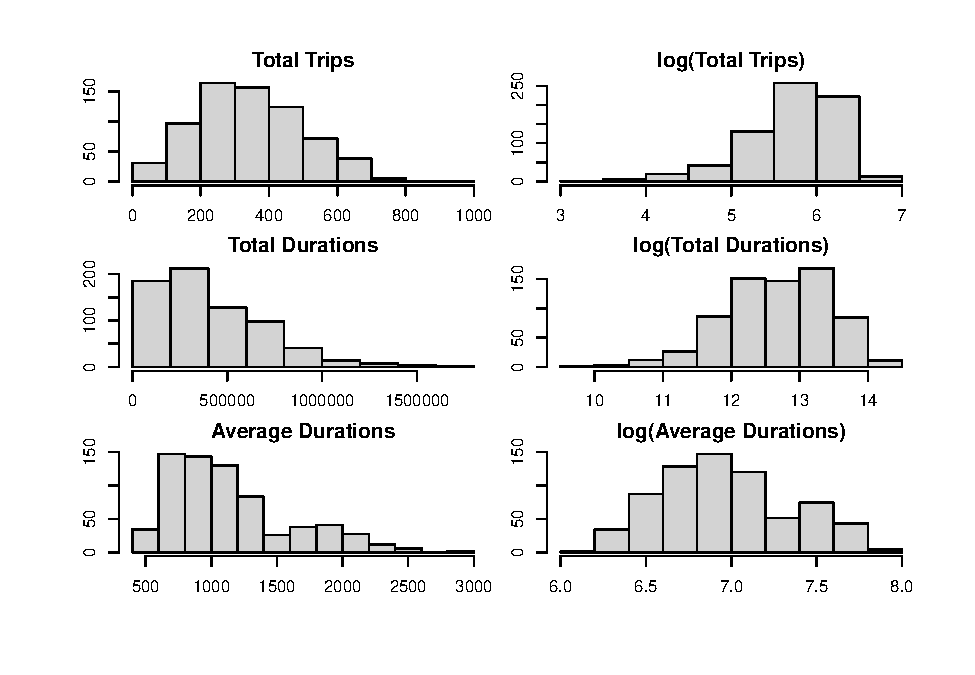
\includegraphics{MATH361_Rough_Draft_files/figure-latex/plot_normal_histograms-1.pdf}

\begin{longtable}[]{@{}lrrr@{}}
\caption{Correlation between Weather Features and Total
Trips}\tabularnewline
\toprule\noalign{}
Feature & Min & Mean & Max \\
\midrule\noalign{}
\endfirsthead
\toprule\noalign{}
Feature & Min & Mean & Max \\
\midrule\noalign{}
\endhead
\bottomrule\noalign{}
\endlastfoot
Temperature (°F) & 0.640 & 0.750 & 0.786 \\
Visibility (miles) & 0.470 & 0.364 & 0.058 \\
Dew Point (°F) & 0.396 & 0.452 & 0.433 \\
Humidity (\%) & -0.648 & -0.680 & -0.579 \\
Sea Level Pressure (in) & 0.180 & 0.079 & -0.065 \\
\end{longtable}

\includegraphics{MATH361_Rough_Draft_files/figure-latex/wind cor plots-1.pdf}
\#\# Outliers

\section{Methods/ Analysis}\label{methods-analysis}

\section{Conclusion/Discussion}\label{conclusiondiscussion}

\subsection{Model Selection}\label{model-selection}

Our model and how we derived it:

The equation for our final regression model is:

\texttt{total\_trips} = 277.1643 -- 4.95(\texttt{Mean\_Humidity}) +
5.90(\texttt{MeanDew\_Point}) -- 118.151(\texttt{Precipitation\_In}) --
7.91(\texttt{Mean\_Wind\_Speed}) + 2.94(\texttt{Max\_Temperature})

Each regressor is significant to at least the 0.01 level, and the
diagnostic plots are satisfactory. The residual plot moving-average
looks flat. The normal quantile plot has few departures from the line.
The scale location plot is relatively flat, indicating constant variance
across fitted values.

In order to obtain this model, we first did some exploratory data
analysis, plotting total trips against certain variables and obtaining
their correlation. We then attemped several basic (single regressor)
linear models of total\_trips vs some of our variables. The variables
that we considered were: mean temperature, mean humidity, mean dew
point, precipitation in inches, mean wind speed, mean miles of
visibility, mean sea level pressure, temperature range, and max
temperature. These were the original variables we considered on account
of the fact that they seemed to have some relationship with total trips
based on plots and correlation, and made sense to us as predictors of
ridership from an intuitive perspective. After trying several single
variable models, we found that few of them had very high R\^{}2, with a
notable exception that a weighted least squares model of wind speed high
worked very well. We then decided to make a ``full'' model with all of
the variables above, except only using mean temperature instead of
temperature range and max temperature as 1. mean and max were extremely
highly correlated (\textgreater97\%) and 2. we thought two temperature
variables would be redundant. The output of the full model showed that
Mean temperature, mean visibility miles, and mean sea level pressure did
not have coefficients that were significantly different from zero. We
made a model dropping these parameters and then did an anova (partial f)
between the two models to see if we could justifiably drop them and it
showed that we could. At this point all of the predictors were
significant and the adjusted R\^{}2 was 0.7095. However, we got the idea
to try adding temperature range or max temperature to this model.
Including temperature range did not improve the R\^{}2, and it was not
significant in the model, however, including max temperature did improve
the adjusted R\^{}2 and the regressor was also significant. We decided
that this would be our final model. Each regressor is significant at at
least the 0.01 level, and the diagnostic plots look good. The adjusted
R\^{}2 is 0.712. We also tried to use powerTransformations, but it only
worked for some of the variables as others did not have strictly
positive values. For the variables that did successfully power
transform, the adjusted R\^{}2 of the subsequent model was not greatly
improved and few of the regressors were significant. Our final model has
some nice properties, in that the diagnostic plots show that it
satisfies the assumptions for linear regression well, it is perfectly
basic in terms of transformations, and partly on account of that, it is
not too difficult to interpret. In terms of interpretation, our model
predicts that holding all else equal, every 1\% increase in average
humidity will lead the total number of bike trips to decrease by 4.95.
It predicts that holding all else equal, for every 1 degree increase in
the average dew point (Fahrenheit for this and all future mentions of
degrees) Seattle will see a drop in bike trips of 5.90. Our model
predicts that all else equal, for every 1 extra inch of precipitation,
total bike rides will drop by 118. It also predicts that holding all
else equal, a 1 mile per hour increase in the average wind speed will
decrease total bike trips by 7.91. Lastly our model predicts that
holding all else equal, a 1 degree increase in the maximum temperature
will increase the number of bike trips by 2.94.

\begin{verbatim}
## 
## Call:
## lm(formula = total_trips ~ Mean_Humidity + MeanDew_Point_F + 
##     Precipitation_In + Mean_Wind_Speed_MPH + Max_Temperature_F, 
##     data = df)
## 
## Residuals:
##     Min      1Q  Median      3Q     Max 
## -232.29  -58.08    0.51   49.71  465.04 
## 
## Coefficients:
##                      Estimate Std. Error t value Pr(>|t|)    
## (Intercept)          277.1643    69.9164   3.964 8.14e-05 ***
## Mean_Humidity         -4.9504     0.7503  -6.598 8.37e-11 ***
## MeanDew_Point_F        5.8968     1.3083   4.507 7.73e-06 ***
## Precipitation_In    -118.1507    15.2166  -7.765 3.00e-14 ***
## Mean_Wind_Speed_MPH   -7.9065     1.2656  -6.247 7.35e-10 ***
## Max_Temperature_F      2.9379     1.1138   2.638  0.00854 ** 
## ---
## Signif. codes:  0 '***' 0.001 '**' 0.01 '*' 0.05 '.' 0.1 ' ' 1
## 
## Residual standard error: 83.09 on 683 degrees of freedom
## Multiple R-squared:  0.7141, Adjusted R-squared:  0.712 
## F-statistic: 341.1 on 5 and 683 DF,  p-value: < 2.2e-16
\end{verbatim}

\includegraphics{MATH361_Rough_Draft_files/figure-latex/final model-1.pdf}
\includegraphics{MATH361_Rough_Draft_files/figure-latex/final model-2.pdf}

\subsection{Cross Validation}\label{cross-validation}

\section{Conclusion}\label{conclusion}

Our work here suggests a path forward for bike share systems looking to
bolster their operations and planning with weather data. However,
Seattle is a city with temperate weather/climate. These results are not
readily generalizable to all cities because when its too hot, people
will also not ride bike!

\section{Appendix}\label{appendix}

\begin{Shaded}
\begin{Highlighting}[]
\NormalTok{trip }\OtherTok{=} \FunctionTok{read\_csv}\NormalTok{(}\StringTok{\textquotesingle{}pronto{-}cycle{-}share{-}trip{-}data.csv\textquotesingle{}}\NormalTok{)}
\CommentTok{\# map unique dates to integers starting at 1}
\CommentTok{\# strips the date from its current format}
\NormalTok{trip}\SpecialCharTok{$}\NormalTok{date }\OtherTok{\textless{}{-}} \FunctionTok{as.Date}\NormalTok{(trip}\SpecialCharTok{$}\NormalTok{starttime, }\AttributeTok{format =} \StringTok{"\%m/\%d/\%Y \%H:\%M"}\NormalTok{) }
\NormalTok{unique\_dates }\OtherTok{\textless{}{-}} \FunctionTok{sort}\NormalTok{(}\FunctionTok{unique}\NormalTok{(trip}\SpecialCharTok{$}\NormalTok{date)) }\CommentTok{\# this collects unique dates}
\CommentTok{\# this maps unique date to the integers, starting at 1}
\NormalTok{date\_to\_number }\OtherTok{\textless{}{-}} \FunctionTok{setNames}\NormalTok{(}\FunctionTok{seq\_along}\NormalTok{(unique\_dates), }\FunctionTok{as.character}\NormalTok{(unique\_dates)) }
\CommentTok{\# this adds the integer mapping as a column, day\_number}
\NormalTok{trip}\SpecialCharTok{$}\NormalTok{day\_number }\OtherTok{=}\NormalTok{ date\_to\_number[}\FunctionTok{as.character}\NormalTok{(trip}\SpecialCharTok{$}\NormalTok{date)] }
\NormalTok{trip}\SpecialCharTok{$}\NormalTok{count }\OtherTok{=} \DecValTok{1} \CommentTok{\# this adds a one to each obs; useful for add}
\NormalTok{trip }\OtherTok{=}\NormalTok{ dplyr}\SpecialCharTok{::}\FunctionTok{select}\NormalTok{(trip, count, tripduration, day\_number)}

\CommentTok{\# construct new df, ridership, that aggregates trips by day}
\NormalTok{ridership }\OtherTok{=}\NormalTok{ trip }\SpecialCharTok{\%\textgreater{}\%} \FunctionTok{group\_by}\NormalTok{(day\_number) }\SpecialCharTok{\%\textgreater{}\%}
  \FunctionTok{summarise}\NormalTok{(}\AttributeTok{total\_trips =} \FunctionTok{sum}\NormalTok{(count),}
            \AttributeTok{total\_durations =} \FunctionTok{sum}\NormalTok{(tripduration),}
            \AttributeTok{.groups =} \StringTok{\textquotesingle{}drop\textquotesingle{}}\NormalTok{); }\FunctionTok{dim}\NormalTok{(ridership)}
\end{Highlighting}
\end{Shaded}

\begin{Shaded}
\begin{Highlighting}[]
\NormalTok{weather }\OtherTok{=} \FunctionTok{read\_csv}\NormalTok{(}\StringTok{\textquotesingle{}weather.csv.xls\textquotesingle{}}\NormalTok{)}
\CommentTok{\# calculates temperature range for each day}
\NormalTok{weather}\SpecialCharTok{$}\NormalTok{temp\_range }\OtherTok{=}\NormalTok{ weather}\SpecialCharTok{$}\NormalTok{Max\_Temperature\_F }\SpecialCharTok{{-}}\NormalTok{ weather}\SpecialCharTok{$}\NormalTok{Min\_TemperatureF }
\CommentTok{\# strips the date from its current format}
\NormalTok{weather}\SpecialCharTok{$}\NormalTok{date }\OtherTok{\textless{}{-}} \FunctionTok{as.Date}\NormalTok{(weather}\SpecialCharTok{$}\NormalTok{Date, }\AttributeTok{format =} \StringTok{"\%m/\%d/\%Y"}\NormalTok{) }
\CommentTok{\# maps unique date to the integers, like the chunk above}
\NormalTok{date\_to\_number }\OtherTok{\textless{}{-}} \FunctionTok{setNames}\NormalTok{(}\FunctionTok{seq\_along}\NormalTok{(unique\_dates), }\FunctionTok{as.character}\NormalTok{(unique\_dates))}
\NormalTok{weather}\SpecialCharTok{$}\NormalTok{day\_number }\OtherTok{=}\NormalTok{ date\_to\_number[}\FunctionTok{as.character}\NormalTok{(weather}\SpecialCharTok{$}\NormalTok{date)]}
\NormalTok{weather }\OtherTok{=}\NormalTok{ weather[,}\SpecialCharTok{{-}}\DecValTok{1}\NormalTok{] }\CommentTok{\# remove the old date}
\CommentTok{\# this will be our data frame going forward}
\NormalTok{df }\OtherTok{=} \FunctionTok{left\_join}\NormalTok{(weather,ridership, }\AttributeTok{by=}\StringTok{\textquotesingle{}day\_number\textquotesingle{}}\NormalTok{); }\FunctionTok{dim}\NormalTok{(df)}
\NormalTok{df}\SpecialCharTok{$}\NormalTok{avg\_durations }\OtherTok{=}\NormalTok{ df}\SpecialCharTok{$}\NormalTok{total\_durations }\SpecialCharTok{/}\NormalTok{ df}\SpecialCharTok{$}\NormalTok{total\_trips}
\end{Highlighting}
\end{Shaded}


\end{document}
